% Options for packages loaded elsewhere
\PassOptionsToPackage{unicode}{hyperref}
\PassOptionsToPackage{hyphens}{url}
%
\documentclass[
  english,
  man]{apa6}
\usepackage{lmodern}
\usepackage{amsmath}
\usepackage{ifxetex,ifluatex}
\ifnum 0\ifxetex 1\fi\ifluatex 1\fi=0 % if pdftex
  \usepackage[T1]{fontenc}
  \usepackage[utf8]{inputenc}
  \usepackage{textcomp} % provide euro and other symbols
  \usepackage{amssymb}
\else % if luatex or xetex
  \usepackage{unicode-math}
  \defaultfontfeatures{Scale=MatchLowercase}
  \defaultfontfeatures[\rmfamily]{Ligatures=TeX,Scale=1}
\fi
% Use upquote if available, for straight quotes in verbatim environments
\IfFileExists{upquote.sty}{\usepackage{upquote}}{}
\IfFileExists{microtype.sty}{% use microtype if available
  \usepackage[]{microtype}
  \UseMicrotypeSet[protrusion]{basicmath} % disable protrusion for tt fonts
}{}
\makeatletter
\@ifundefined{KOMAClassName}{% if non-KOMA class
  \IfFileExists{parskip.sty}{%
    \usepackage{parskip}
  }{% else
    \setlength{\parindent}{0pt}
    \setlength{\parskip}{6pt plus 2pt minus 1pt}}
}{% if KOMA class
  \KOMAoptions{parskip=half}}
\makeatother
\usepackage{xcolor}
\IfFileExists{xurl.sty}{\usepackage{xurl}}{} % add URL line breaks if available
\IfFileExists{bookmark.sty}{\usepackage{bookmark}}{\usepackage{hyperref}}
\hypersetup{
  pdftitle={Toward a Framework for Collaboratively Writing Open Books in Education},
  pdfauthor={Joshua Rosenberg1, Isabella C. Velásquez2, , Jesse Mostipak2, , Emily A. Freer2, \& Ryan A. Estrellado2},
  pdflang={en-EN},
  pdfkeywords={keywords},
  hidelinks,
  pdfcreator={LaTeX via pandoc}}
\urlstyle{same} % disable monospaced font for URLs
\usepackage{graphicx}
\makeatletter
\def\maxwidth{\ifdim\Gin@nat@width>\linewidth\linewidth\else\Gin@nat@width\fi}
\def\maxheight{\ifdim\Gin@nat@height>\textheight\textheight\else\Gin@nat@height\fi}
\makeatother
% Scale images if necessary, so that they will not overflow the page
% margins by default, and it is still possible to overwrite the defaults
% using explicit options in \includegraphics[width, height, ...]{}
\setkeys{Gin}{width=\maxwidth,height=\maxheight,keepaspectratio}
% Set default figure placement to htbp
\makeatletter
\def\fps@figure{htbp}
\makeatother
\setlength{\emergencystretch}{3em} % prevent overfull lines
\providecommand{\tightlist}{%
  \setlength{\itemsep}{0pt}\setlength{\parskip}{0pt}}
\setcounter{secnumdepth}{-\maxdimen} % remove section numbering
% Make \paragraph and \subparagraph free-standing
\ifx\paragraph\undefined\else
  \let\oldparagraph\paragraph
  \renewcommand{\paragraph}[1]{\oldparagraph{#1}\mbox{}}
\fi
\ifx\subparagraph\undefined\else
  \let\oldsubparagraph\subparagraph
  \renewcommand{\subparagraph}[1]{\oldsubparagraph{#1}\mbox{}}
\fi
% Manuscript styling
\usepackage{upgreek}
\captionsetup{font=singlespacing,justification=justified}

% Table formatting
\usepackage{longtable}
\usepackage{lscape}
% \usepackage[counterclockwise]{rotating}   % Landscape page setup for large tables
\usepackage{multirow}		% Table styling
\usepackage{tabularx}		% Control Column width
\usepackage[flushleft]{threeparttable}	% Allows for three part tables with a specified notes section
\usepackage{threeparttablex}            % Lets threeparttable work with longtable

% Create new environments so endfloat can handle them
% \newenvironment{ltable}
%   {\begin{landscape}\begin{center}\begin{threeparttable}}
%   {\end{threeparttable}\end{center}\end{landscape}}
\newenvironment{lltable}{\begin{landscape}\begin{center}\begin{ThreePartTable}}{\end{ThreePartTable}\end{center}\end{landscape}}

% Enables adjusting longtable caption width to table width
% Solution found at http://golatex.de/longtable-mit-caption-so-breit-wie-die-tabelle-t15767.html
\makeatletter
\newcommand\LastLTentrywidth{1em}
\newlength\longtablewidth
\setlength{\longtablewidth}{1in}
\newcommand{\getlongtablewidth}{\begingroup \ifcsname LT@\roman{LT@tables}\endcsname \global\longtablewidth=0pt \renewcommand{\LT@entry}[2]{\global\advance\longtablewidth by ##2\relax\gdef\LastLTentrywidth{##2}}\@nameuse{LT@\roman{LT@tables}} \fi \endgroup}

% \setlength{\parindent}{0.5in}
% \setlength{\parskip}{0pt plus 0pt minus 0pt}

% \usepackage{etoolbox}
\makeatletter
\patchcmd{\HyOrg@maketitle}
  {\section{\normalfont\normalsize\abstractname}}
  {\section*{\normalfont\normalsize\abstractname}}
  {}{\typeout{Failed to patch abstract.}}
\patchcmd{\HyOrg@maketitle}
  {\section{\protect\normalfont{\@title}}}
  {\section*{\protect\normalfont{\@title}}}
  {}{\typeout{Failed to patch title.}}
\makeatother
\shorttitle{Open Book}
\keywords{keywords\newline\indent Word count: X}
\DeclareDelayedFloatFlavor{ThreePartTable}{table}
\DeclareDelayedFloatFlavor{lltable}{table}
\DeclareDelayedFloatFlavor*{longtable}{table}
\makeatletter
\renewcommand{\efloat@iwrite}[1]{\immediate\expandafter\protected@write\csname efloat@post#1\endcsname{}}
\makeatother
\usepackage{lineno}

\linenumbers
\usepackage{csquotes}
\ifxetex
  % Load polyglossia as late as possible: uses bidi with RTL langages (e.g. Hebrew, Arabic)
  \usepackage{polyglossia}
  \setmainlanguage[]{english}
\else
  \usepackage[shorthands=off,main=english]{babel}
\fi
\ifluatex
  \usepackage{selnolig}  % disable illegal ligatures
\fi
\newlength{\cslhangindent}
\setlength{\cslhangindent}{1.5em}
\newlength{\csllabelwidth}
\setlength{\csllabelwidth}{3em}
\newenvironment{CSLReferences}[2] % #1 hanging-ident, #2 entry spacing
 {% don't indent paragraphs
  \setlength{\parindent}{0pt}
  % turn on hanging indent if param 1 is 1
  \ifodd #1 \everypar{\setlength{\hangindent}{\cslhangindent}}\ignorespaces\fi
  % set entry spacing
  \ifnum #2 > 0
  \setlength{\parskip}{#2\baselineskip}
  \fi
 }%
 {}
\usepackage{calc}
\newcommand{\CSLBlock}[1]{#1\hfill\break}
\newcommand{\CSLLeftMargin}[1]{\parbox[t]{\csllabelwidth}{#1}}
\newcommand{\CSLRightInline}[1]{\parbox[t]{\linewidth - \csllabelwidth}{#1}\break}
\newcommand{\CSLIndent}[1]{\hspace{\cslhangindent}#1}

\title{Toward a Framework for Collaboratively Writing Open Books in Education}
\author{Joshua Rosenberg\textsuperscript{1}, Isabella C. Velásquez\textsuperscript{2}, , Jesse Mostipak\textsuperscript{2}, , Emily A. Freer\textsuperscript{2}, \& Ryan A. Estrellado\textsuperscript{2}}
\date{}


\authornote{

Enter author note here.

Earlier draft: \url{https://docs.google.com/document/d/1Z0u0A25noHq-ioKVyDp94BVqNQW-siKi3QvQDad5rTQ/edit\#}

Correspondence concerning this article should be addressed to Joshua Rosenberg, Postal address. E-mail: \href{mailto:my@email.com}{\nolinkurl{my@email.com}}

}

\affiliation{\vspace{0.5cm}\textsuperscript{1} University of Tennessee, Knoxville\\\textsuperscript{2} }

\abstract{
In this paper, we discuss the benefits of writing an open, technical book in educational settings.
}



\begin{document}
\maketitle

In 2017, we started work on our book, Data Science in Education Using R (DSIEUR). We had two goals for DSIEUR. First, we aimed to write a practical reference for data scientists in education that helps them learn and apply R skills in their jobs. Second, we wanted to share the process with the R community by writing the book in the open on GitHub.

There are new books being written in and about education all of the time, yet, what is less typical was the second of our two goals, writing and sharing our book in the open. The reason for this focus is that this part of the process came naturally to us: sharing our work openly was and is a norm in the data science (and the nascent educational data science) community. Yet, at the same time, this was the part of our process that was the least-specified, in that we didn't have clear guidelines or expectations from the outset for how we would do this.

Moreover, this goal - sharing the book in the open - was the part that still fascinated us after publishing the book. Why, for instance, did our publisher allow us to share our book in this way? What benefits did this mode of producing a book have? And, what might this work have to say about broader conversations in educational research open science (see Van der zee \& Reich, 2018)?

In this article, we attempt to step back from writing the book to describe our process for sharing in the open. In doing so, we aim to generalize from our experiences, and also speak to what we think the implications of this model of sharing scholarly work in education might mean. We focus on what we call the open-source authorship process we took to write the book. We think of open-source authorship as a broader---and perhaps better---term for describing what authors of some open books undertake. Thus, our goal is to write an article that draws on these areas of past research to articulate this framework to describe what we did. In doing so, we provide a description and examples for each component and describing the implications in terms of our own book. We conclude with the wider implications of this work.

\hypertarget{prior-research-scholarship-and-development-related-to-open-source-authorship}{%
\section{Prior Research, Scholarship, and Development Related to Open-Source Authorship}\label{prior-research-scholarship-and-development-related-to-open-source-authorship}}

In our use and characterization of it, the open-source authorship process draws upon a) parts of open-source software (OSS) values and tools, b) parts of open science that establish the importance of scholarly work beyond original, discovery research, and c) the values surrounding the creation of open educational resources (OER). We believe that combining elements from OSS, open science, and OER is notable because while OSS and open science emphasize the sharing of technical work (including technology and code) and OER emphasizes the sharing of resources, technical books have not been as much a focus of the conversation. We think that combining these has merit, and also that not combining them can lead to some negatives: not considering these different ideas and efforts when writing an open book might mean that those involved with OSS development and open science may fail to recognize the creation of a book as a substantial contribution. In this way, we argue for open-source authorship as an important, new type of work, one that we increasingly see by the authors of other books, especially in the computer science and data science disciplines (see Xie et al., 2020; Lovelace et al., 2020; Wickham, 2020; Wickham \& Grolemund, 2017; Navarro, 2020).
Originally a niche effort, open-source software (OSS) and OSS development are (likely not to the surprise of R users!) now widespread (DiBona \& Ockman, 1999; Eghbal, 2020). There are some insights that can be gained from efforts to understand how OSS development proceeds. For example, in foundational, work Mockus et al.~(2002) found that OSS is often characterized by a core group of 10-15 individuals contributing around 80\% of the code, but that a group around one order of magnitude larger than that core will repair specific problems, and a group another order of magnitude larger will report issues; proportions (generally) similar to those we found for those who contributed to our book.

Second, open science is both a perspective about how science should operate and a set of practices that reflect a perspective about how science should proceed (National Academies of Science, Engineering, and Medicine, 2018; van der Zee \& Reich, 2018). Related to open science are open scholarly practices. Others (see Greenhow \& Robelia, 2009; Greenhow et al., 2019) trace the origin of the idea of open scholarly practices to a book by Boyer (1990), who shared a broad description of intellectual (especially academic) work. This suggests that scholarly work is not only original, discovery research; it also includes the applications of advances in one's own discipline (or ``translational research'') and sharing the results of research with multiple stakeholders. Open science and open scholarly practices point to the scientific or scholarly contributions of open books; while different from original, scientific research, books such as our own---which focused on providing a language for data science in education---may serve as helpful examples (of open science) or forms of a broader view of scholarship.

Last, OER are ``teaching, learning, and research resources that reside in the public domain or have been released under an intellectual property license that permits their free use and re-purposing by others'' (William and Flora Hewlett Foundation, 2020). These resources range from courses and books to tests and technologies. By being open, they are not only available to others to use, but also to reuse, redistribute (or share), revise (adapt or change the work), and remix (combining existing resources to create a new one) (Hilton et al., 2010). OER can serve as an inspiration for authors of open books, especially those who see their books as being used to teach and learn from. In addition, a number of platforms for creating books that are OER are emerging; one example is EdTech Books (EdTech Books, 2020). There are increasing conversations related to making materials, resources, and even education as an enterprise more open; OER may be an area in which authors of books about R and other technical books can both learn from the work of authors as well as advance the conversation.

\hypertarget{a-framework-for-collaboratively-writing-an-open-book}{%
\section{A Framework for Collaboratively Writing an Open Book}\label{a-framework-for-collaboratively-writing-an-open-book}}

Our framework for collaboratively writing an open book is presented in Figure 1. In this framework, processes are depicted as circles; products as rectangles.

\begin{figure}
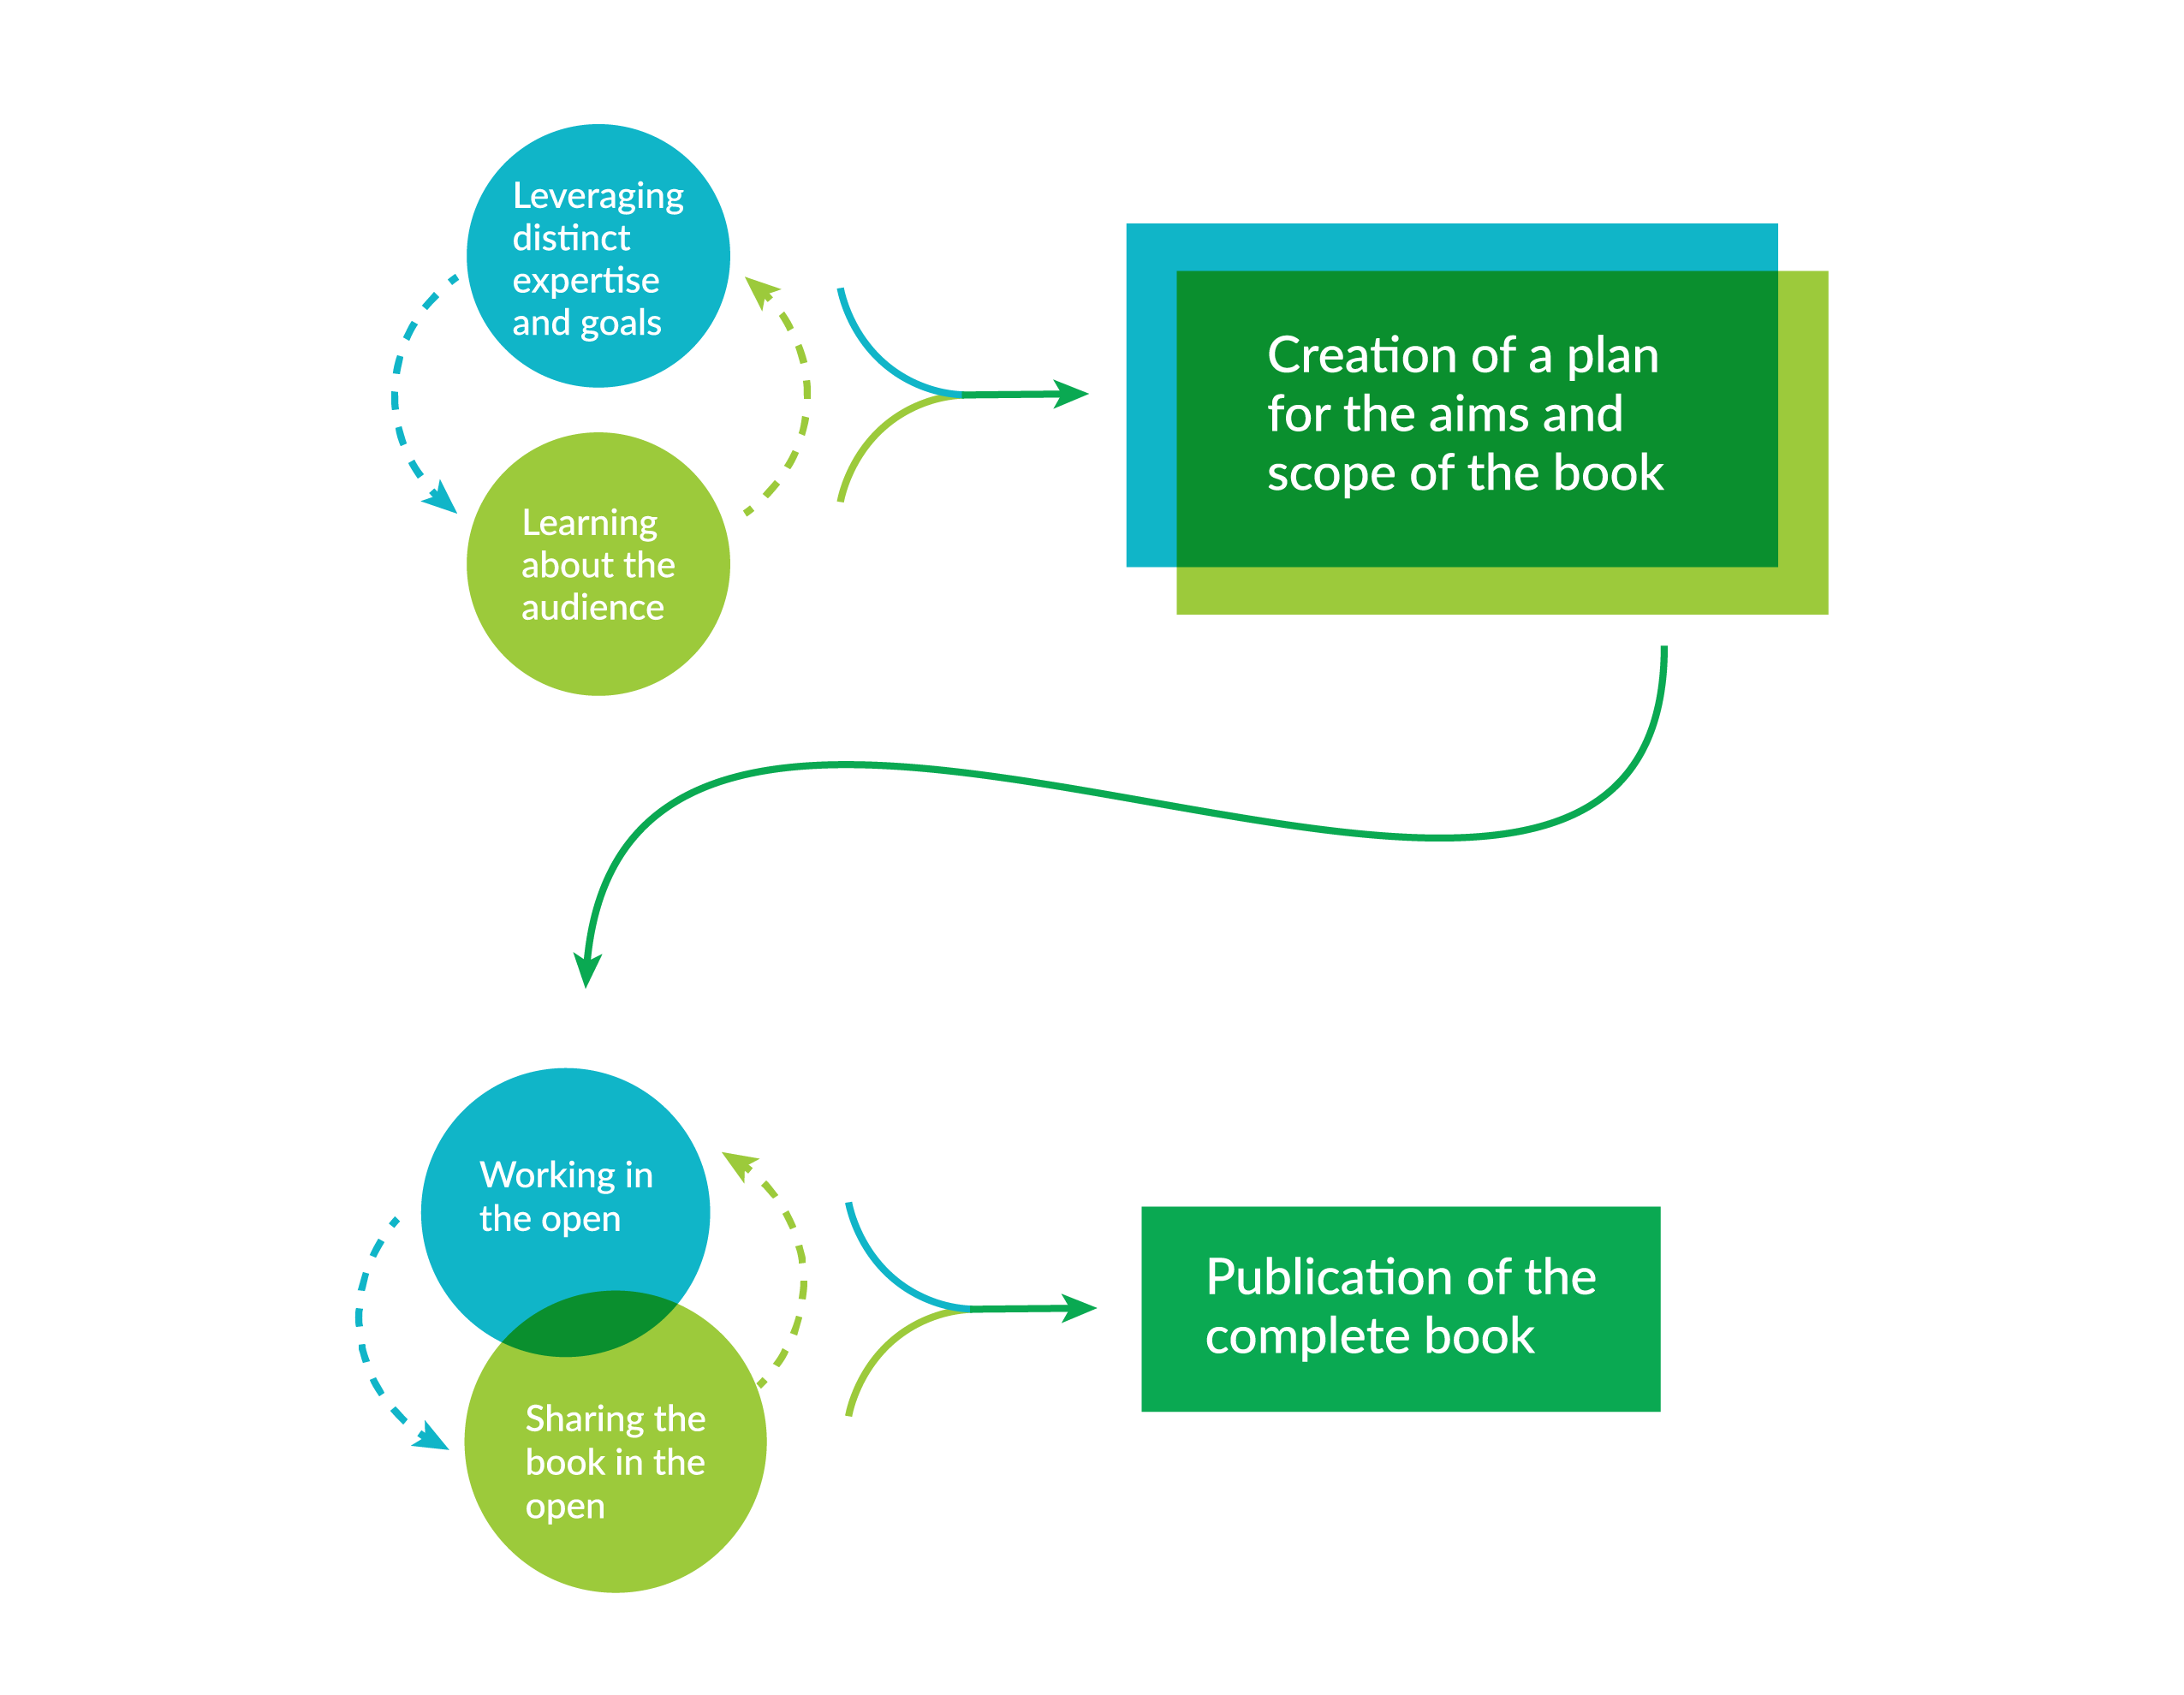
\includegraphics[width=8.5in]{framework-diagram} \caption{ }\label{fig:unnamed-chunk-1}
\end{figure}

First, two planning-related processes--leveraging distinct expertise and goals and learning about the audience--lead to and are encapsulated in a plan for the book--and, writing this plan can shape what expertise is leveraged and who the audience is. These are bidirectionally related; learning about the audience can, for instance, shape what expertise the authors choose to draw upon.

Then, the processes of working and sharing in the open lead to the publication of the complete book; knowing that the book will be published, and published in a particular form, impacts how work is done in the open, and how this work is shared. Again, these processes are bidirectional, in that feedback received through sharing in the open can inform the process of working in the open; and, knowing that work will be shared in the open can shape the nature of the work of creating the book.

In the following subsections, we elaborate on each of the aspects of this framework, providing examples from our own work within each.

\hypertarget{leveraging-distinct-expertise-and-goals}{%
\subsection{Leveraging Distinct Expertise and Goals}\label{leveraging-distinct-expertise-and-goals}}

Academics are used to working collaboratively, but, particularly for multiple authors, co-authorship is less common, with one (or two) authors typically taking the lead. For collaborative books, however, collaborative authorship has value in that it allows for authors to take ownership of different parts of the process, more akin to how large grant-funded projects are coordinated by multiple individuals. We think that this latter model is better for book projects in that it allows for distinct expertise and goals to be leveraged--and that doing so improves the work.

We focus on three ways that distinct expertise and goals can be leveraged that emphasize being open and inclusive while also having a clear sense for what being an author entails, recognizing the value in different skills and expertise, different means of contributing

\emph{Having an open call for authors, but also having clear guidelines for what it means to be in.}

Our project started in an atypical way: through an affinity group (Gee et al., 20xx) for individuals interested in educational data science. In this group, we shared and discussed about the value and challenges of doing data science in education. At some point, members began discussing creating resources for others interested in the topic. This led to a number of meetings (organized via Zoom) open to anyone interested in the topic. In these meetings, we discussed writing a book, and, later, asked widely of group members about their interest in writing the book. This open call led to five authors who committed to this project - and, a number of other members who could or did not commit to writing the book, but were, nevertheless, interested in supporting the book in other ways, such as by auditing code included in the book. In this way, we think that having an open call for authors, and being inclusive of anyone interested, while also having clear guidelines for what it means to contribute, was important.

\emph{Allowing authors to focus on content that suits their expertise.}

Early in our project, we decided that we would let each author focus on topics and aspects of the writing process where they felt strongest. Each author could lead writing in areas of strength and take a supporting role on other chapters. Additionally, some authors felt strongly about the narrative, whereas others felt strongly about the code performance or about addressing the audience's needs. We could agree that it was important to balance all of these things, but no single one of us could have effectively addressed them all.

Another side of this value manifested later in the project, with respect to how we wove together our different contributions. As we neared the end of writing the DSIEUR manuscript, we set out to review each chapter and edit it for readability. To create an opportunity for fresh eyes to read our work, we each reviewed a chapter we hadn't written. Ryan picked chapter 13, which is on using multilevel models to analyze student survey responses about their online classes. Having a new perspective on experiencing the chapter---particularly when the chapter includes lots of technical explanations---turned out to be a great way to discover blind spots in our work. Here were Ryan's thoughts after reviewing chapter 13:

``I don't use multilevel models regularly in my work, so I could tell right away I was going to learn something new. I read through the sections to make small edits, but also took breaks every so often to check my comprehension of the concepts.''
About halfway through the chapter review, we started a great, back-and-forth conversation and brainstorm about conveying how standardizing coefficients works in multilevel models. Thinking back, we see that our different experiences with multilevel models were critical for accomplishing two things: identifying areas where the writing could be clearer and more accessible and also staying true to the technical parts of the topic.

We read through the chapter and picked out sections that didn't seem clear. Then, we had conversations to clarify how standardizing coefficients work in multilevel models. We wrote out some initial thoughts to convey where we-together-ended up in our conversation. Then, we read the section again. And round and round we went, until finally we arrived at an execution we were happy with.

In this way, we supercharged the iterative writing process with two elements of collaboration. First, differing backgrounds gave us an opportunity to find blind spots. Josh has used, taught, and written about multilevel models regularly for years. Ryan had a basic understanding of the concepts, but less experience using them. And second, a collective goal---in this case, writing a book together---motivated us to communicate openly and experiment with different ways to create a great experience for our readers.
Allowing authors to focus on means of contributing

In addition to allowing authors to leverage their expertise, we also considered the different ways one could contribute. Isabella, for example, built all the technical infrastructure for the book, including our use of Bookdown and also the R package that accompanied the book. Different authors took, at different points, the lead on communication with the publisher and advertising the book. Finally, nearer the end, different authors prioritized different aspects of the editing process, with some being focused on the technical rigor of the statistical code, and others focusing on the arc and narrative of the book, particularly for newcomers. Allowing authors to contribute in different ways was a way to leverage our backgrounds--and improve the book.

\hypertarget{b.-learning-about-the-audience}{%
\subsection{1b. Learning About the Audience}\label{b.-learning-about-the-audience}}

Educators and educational researchers are familiar with the maxim to know one's students. Research has shown that knowing about students' ideas can help them to serve as resources for instructors (CITE). When it comes to writing, the same is true: keeping one's audience in mind can XXX (CITE). When it comes to writing a book on a new topic, though, who the audience is and what they know and value are less clear, and, so, learning about the audience is also important.

In this section, we describe how we aimed to provide a grammar for educational data science, constructed reader personas, and engaged our audience (and potential readers and contributors) early in the writing process.

\emph{Providing a language for data science in education}

Discovering a new R concept like a function or package is exciting. You never know if you're about to learn something that fundamentally changes the way you code or solve data science problems. Still, for most people using R in their jobs, there's another step. They have to imagine how to apply what they've read and seen to the problems they're solving at work. But what if we used education datasets to help them imagine using R on the job, just as the authors of ISL use words and code to teach about models and Julia Silge uses video to inspire coding?

We learned from writing DSIEUR that we can combine words, code, and professional context. Professional context includes scenarios, language, and data that readers will recognize in their education jobs. We wanted readers to feel motivated and engaged by seeing words and data that reminds them of their everyday work tasks. This connection to their professional lives is a hook for readers as they engage R syntax which is, if you've never used it, literally a foreign language.

As an example of this, a common data structure in education is one in which assignments, or questions, are represented in spreadsheet columns, with students' responses in rows (``wide'' format data); however, a different data structure is often needed for modeling and visualizing data, ``long'' format data. When we introduced transforming data from wide to long format, we did so in the context of familiar educational data, and set the stage for why one would collect data in wide format, but transform it in long format.

\emph{Constructing personas}

We constructed personas representing different types of readers in our audience. To do so, we identified the categories of skill that we thought were germane to audience members: programming, stats, and education experience (Conway et al., 2004; Rosenberg et al., 2020). Then Jesse fiddled with the knobs on each of these to make different reader profiles (and associated Hamilton names), until we settled on personas. We then identified questions that we had as authors based upon these personas; specifically, how the book could meet their needs.

As an example, here was one persona:

\begin{quote}
Angelica has worked as an analyst in her district for five years, primarily using Excel, STATA, and PowerBI. She loves trying new technologies and software. The bulk of her work is spent creating dashboards and writing summary statistics reports on standardized tests and accountability data, and she's tried R because of the graphing capabilities. Her team consists of three other analysts who work on similar data, and her organization has additional analytical teams focused on other areas of education, including teacher and principal retention and quality, school culture and climate, and student enrollment. All teams across the organization use the same tools, so her interest in R is largely a solo endeavor.
\end{quote}

This raised the question: ``Should we have an introductory chapter on Shiny, for example rapid prototyping?''

Here is another example:

\begin{quote}
Thomas has a degree in Biology and started teaching three years ago. He has used Excel to track student grades and successfully implement targeted instructional interventions. Because of this, his Principal has asked him to take on the new role of ``data lead,'' where he will use data to target interventions for the entire 10th grade teaching team. He's suddenly responsible for wrangling and analyzing gradebooks from 15 teachers and finding that Excel - his favorite tool - isn't quite up to the task. His Principal gave him the book, ``Data Science in Education with R'' as a resource (which he heard about at a conference), but Thomas has no idea where to start.
\end{quote}

This raised the questions: 1) Should we build out the gradebook chapter to include the scenario of wrangling multiple Excel sheets that are formatted differently (in addition to the current gradebook)? And 2) What kind of guidance should we provide at the start of the book? Would it be helpful to share user personas in order to guide readers on chapter selection?

\emph{Engaging our audience early on social media}

Using social media was a substantial part of the work of writing our book, and, especially, engaging our audience. We shared about our intent to write a book and plans and ideas early in the process; doing so helped us substantively (as we had an audience who we could turn to with questions and input) as well as in a more social way (as we had encouragement and accountability).

\hypertarget{creation-of-a-plan-for-the-aims-and-scope-of-the-book}{%
\subsection{2. Creation of a Plan for the Aims and Scope of the Book}\label{creation-of-a-plan-for-the-aims-and-scope-of-the-book}}

Academics are used to developing projects in stages: begin with a conference presentation, progress to a journal; article, and, later, possibly expand the work (and repeat the process) with a follow-up study; books, though, do not have such a natural progression, apart from a proposal for the book which can serve as a plan for its aims and scope. When starting to write a book, particularly one that is open, it is tempting to begin writing, and to allow the book to develop on its own. However, we found that coming up with a plan was not just busy work that was necessary to propose the book to a publisher (though it was helpful for that goal); it was also helpful for clarifying our ideas about the book, its aims, and what its scope would be, all in light of our expertise and audience. In this way, this step captured the results of leveraging our expertise and learning about our audience.

In this section, we describe how articulating our aims more clearly helped us to focus, and narrow, the scope of the book, layout the chapters in a careful way, and summarize the unique contributions of the book.

\emph{Focus on our audience and the scope of the book}

First, articulating our aims helped us to narrow our focus. Initially, we considered writing a book for researchers, analysts or evaluators, and teachers--and maybe even for students interested in the topic! As we discussed not only our aims but also how the book would be organized, it became evident that this focus was too broad: we needed to target a more specific audience well. Our compromise was not to focus only on analysts, but to focus on researchers, analysts or evaluators who work with data; and to acknowledge that while administrators and teachers may use this book, that it is not as tailored to their work (though one of us is writing such a book now; see Estrellado et al., under contract). Moreover, while we chose not to focus on teachers (r learners), we included a chapter on teaching data science that is relevant to researchers and analysts (including faculty who may be teaching data science courses, or anyone teaching a peer in a mentoring or one-on-one context).

\emph{Layout of the chapters}

Laying out the chapters and their organization helped us to think about what our goals were, and how the book could meet them. Specifically, we laid out two sets of objectives, those more conceptual in nature and those more skills-based and applied:

By the end of this book the reader will understand:
- The diversity of data analysis skills and applications in the education field\\
- The unique challenges that come with analyzing education data\\
- That good data analysis has a basic workflow and how they might implement such a workflow\\
- The wonderful opportunity we have to shape the usefulness of data science in our education jobs

And, the reader will be able to:

\begin{itemize}
\tightlist
\item
  Reflect and determine what their role is as a data analyst within their role as an educator\\
\item
  Identify and apply solutions to education data's unique challenges, such as cleaning datasets and working with private student data\\
\item
  Apply a basic analytic workflow through practice with education datasets\\
\item
  Be thoughtful, empathetic, and effective when introducing data science techniques in their education jobs
\end{itemize}

We ended up organizing the book into three sections, two of which were more conceptual in their content (the first and third), and one which drew from the tutorials common to the computer science and programming worlds (and the gaming worlds), walkthroughs (the second):

\begin{itemize}
\tightlist
\item
  An overview of what data science in education is and why it is important (i.e., how data science ideas are relevant to education and what challenges are faced by those doing data science in education).
\item
  An education-focused introduction to a widely-used, freely-available statistical open source software tool, R, and walkthroughs for how R can be used to achieve data and data analysis-related goals.
\item
  A discussion of what to do once one has a foundation in using data science, including tips on how to be strategic about implementing data science and how educators and education consultants can teach others to use data science tools and methods.
\end{itemize}

\emph{Articulation of the summary of the book that helped us to get our thinking on the page}

A principle of science teaching is that putting ideas to the page can be instructive to the (learner) doing so, and can also provide access to others to those ideas--and to critique and improve them. Writing even a title and an abstract for the book, even at this early stage, made the work more concrete and gave us a language to describe the book. This (see below) helped us at multiple stages; having a concise summary of the book, like that we wrote below, helped us to share about what we were doing in a cohesive way; this content also later was able to be edited to work for promotional material. In sum, this part of writing the plan for the book, something not all authors of open books may do, gave us something akin to a mission statement to organize our work around.

This book aims to give data science in education a common language and set of skills so that the community around this topic can grow and learn more together. It is a friendly welcome to educators who are interested in exploring techniques for data analysis in education. It adds to the growing body of data science books by demonstrating data science using the language, datasets, problems, and workflows that are specific to education. It aims to help educators move from ``knowing about'' data analysis tools to ``knowing how to'' conduct meaningful data analyses in their work. This book is ideal for educators at all grade levels looking to start exploring how to use data science in their everyday work, educators who are looking to level up their use of data by learning about programming and machine learning, data-savvy consultants who help educators meet their goals, or experienced data scientists looking for hands on examples that are directly from the education field.

\emph{Express our aims with respect to how the book would be published}

A final benefit of the plan was that it served as a proposal, and it allowed us to make the case to a publisher that writing the book in the open was natural and mutually beneficial. At the moment, OER and traditional publishing modes are largely separate: For most books that are published, the publisher retains the copyright, and authors are typically not allowed to share their book in the open, though this may be changing. Many authors of books about R have negotiated with their publisher to share their books in the open (often only as a website, as we have) in addition to sharing them through print and e-book formats. We were able to layout in the proposal the benefits of open work, and to ask our publisher about whether we could, like other authors of R books, publish a version of our book in the open, which they agreed to do.

\hypertarget{a.-working-in-the-open}{%
\subsection{3a. Working in the Open}\label{a.-working-in-the-open}}

Asdf

Illustrations

\emph{Writing via GitHub in a way that allowed others to help us to improve the writing}

\emph{Creating an R package}

\emph{Bookdown and netlify as an accessible way to share; also an email address}

Early in our process, we determined that we wanted to share the book in an open way. Since we were using GitHub as a repository for the book, it was easy for the contents of the book to be available for anyone to view--even before and as the book was being written. Despite the benefits of using GitHub, GitHub can be difficult to navigate for those who are unfamiliar with it, and so sharing the book in a more widely-accessible way was also important. To do this, we used \{bookdown\} and Netlify to share the book as a website. Additionally, we chose an easy-to-remember URL (\url{http://datascienceineducation.com/}) to help others (and us!) to be able to access it easily.

There are all kinds of ways to build empathy for new learners, like ``listening'' on social media, interviewing members of the community/practice/context you are studying, and regularly trying to learn new things ourselves. Open source educational resources, software, and science make code available to readers to encourage collaboration and accountability. But can open source writing also help us check our biases about what learners need by including the learners themselves in the development of the content?

When data scientists share their writing and code through sites like GitHub and Kaggle, that sharing comes with an unspoken invitation to communicate with the creators. Most of the time, that communication is about improving code. When the open source project is designed to teach something new, the communication can also be about improving the learning experience.

Consider a scenario where a classroom teacher asks their students to complete worksheets---an example of (tacitly) closed source education materials. Not only do worksheets hide the underlying thinking behind their creation: they also invite compliance more than they invite conversation about what the learner needs.

On the other hand, providing the code for our book at every stage of writing empowered us to share how we thought through an analysis. It also set the tone for conversation on social media platforms and GitHub about how we can improve the book. For example, in Chapter 8 we created a visualization to explore scores from student classwork assignments. For this post, we added reorder() to change the order of values in the x-axis:

By making the code for this plot available, we implicitly invited readers (implicitly by being openly available but also explicitly by requesting feedback on Twitter) to tell us where we could do more to scaffold the lesson. For example, a reader might tell us they need more explanation of how reorder() is used to arrange the boxplots by median scores.

Lastly, we shared products that could be seen as tangential to the book, but which were important given its focus on data science and R. Namely, we created an R package, \{dataedu\}, to accompany the book. This package includes code to install the packages necessary to reproduce the book as well as all of the data sets used in it. By doing so, we invited others to contribute to the book in ways not related to its prose. This also led to (pleasantly) surprising contributions, including the creation of an iPython Notebook with python code to carry out comparable steps as those carried in a walkthrough chapter of our book.

\hypertarget{b.-sharing-the-book-in-the-open}{%
\subsection{3b. Sharing the Book in the Open}\label{b.-sharing-the-book-in-the-open}}

Asdf

Illustrations

\emph{Asking for help and defining goals}

\emph{Getting asked to elaborate on our work - blog posts, talks}

\emph{Sharing periodic goals}

As someone who started following the R community on Twitter after it was already well established and popular, I never felt the apprehension about having to ask how to get involved or interact with others. First, there are so many avenues. The R community offers many ways to let you in, whether it be replying to tweets, posting a question on community.rstudio.com, or sharing a blog post on R Weekly. Second, the R community welcomes users no matter their level. Whether it is a code snippet with a function you found cool, a blog post, or a personal side project, there are ways to engage that appeal to everybody. Members of the R community can interact how they want and as often as they want. For us, it was exciting to meet on Twitter, talk about collaborating on an education data project, and then just get started on it. We felt welcome and encouraged to do so. Because people in the R community meet other users virtually and begin side projects all the time, we didn't have to worry about whether something like this was possible: The invitation was already there.

The R community offers so many opportunities to get feedback, advice, and information from a wide variety of users. Early on in the book development, we had a lot of questions to nail down: who is the audience? ``Data is'' or ``data are?'' How do we describe ``people who work in the education field and use data and want to get more effective at it?'' Finding a common language was difficult, but we were able to do this by engaging others in the wider R community. We listened to the stories of many data scientists who work in education, then found common experiences we could describe in our writing. As an example, we learned we weren't the only ones challenged by learning a programming language while attending to full time jobs and personal lives. Knowing this, we made sure to discuss these challenges in our book and offer various ways of engaging with the material based on the reader's needs.

Throughout the process of writing DSIEUR, we asked the R community several times for other types of feedback and suggestions. We also ran into some technical issues, especially when it came to preparing our manuscript with \{bookdown\} to meet our publisher's specifications, and were able to get ideas on how to resolve them. We know that the R community is a safe and encouraging place to ask questions, and this enabled us to write a stronger book.

The community participation throughout the DSIEUR process helped us define our goals and get feedback. Another wonderful aspect is that the R community engaged us back. Writing this R Views series is an example: Someone reached out to us and wanted us to reflect on what we discovered and share it with all of you. This type of engagement reminds us of what an inclusive and encouraging place the R community is and helps us come up with new ways of making sure others see the invitation as well.

In other cases, readers let us know when the writing itself didn't make sense. For example, one community member read the online version of DSIEUR and emailed to tell us a plot that showed the importance of different variables for predicting a student's final grade didn't match the interpretation we wrote. It turns out we made revisions to the analysis that changed the plot, but we hadn't updated the plot's interpretation. We tracked this feedback and others in a GitHub issue and corrected it.

One way to do this is to write for an audience (of any size). If you've written a blog or social media post before, you might recognize the experience of doing so: As soon as you publish the post, you find gaps (or typos!) in your writing you feel motivated to fix. Moreover, if you write a blog post in R Markdown, the process of publishing the post will expose issues, warnings, or messages related to the code---issues you may wish to address before (or after) publishing the post. Knowing someone will read your work gives that extra bit of productive pressure to offer value to your readers. Indeed, the audience has a role to pay in the creative process because they aren't just reading, they're participating. Conversations can start in the comment section or on social media. These conversations help you learn how well you've connected with the audience and help you uncover what's important to your readers.

\hypertarget{publishing-the-book}{%
\subsection{4. Publishing the Book}\label{publishing-the-book}}

Asdf

\emph{Deadlines}

\emph{Reviewing ourselves}

\emph{Reviewing by others}

Another part of structuring creative endeavors is creating opportunities to have your work reviewed, either by you or by someone else. In the context of book writing, working through the copy-edits with our publisher helped (or forced!) us to encounter other parts of our writing we hadn't considered: We realized late in the process that we used both the singular and plural form of `data' throughout the manuscript (without expressed reasons for doing so!). Even an early GitHub issue about this very topic hadn't prompted the same level of urgency as the copy-edits did. While more particular than the broader blind spots discovered through collaboration and writing in the open, these blind spots are critical for creating a clear, professional, and readable book for the audience. Whether reviewing your own work or having others review for you, an intentional revision process can uncover missed opportunities for improvements.

Finally, deadlines can help. The due date for the manuscript motivated us to improve how we communicated with each other. When we structure our creative endeavors like a formal project---including setting a deadline and working toward a product---we create many opportunities to encounter our oversights and blind spots.

Indeed, the frequency of team calls and the commitment to revising and finalizing our manuscript together grew as our deadline approached. Thus, our publisher's deadline provided a structure that encouraged organization, efficient decision-making, problem-solving, and collaboration. With the deadline looming, we got to the essential question as quickly as possible: Does what we wrote connect meaningfully with the audience and if not, how can we speak to them better?

It was a pivotal moment when we decided that we were allowed to edit each other's words without first asking permission. Prior to this point, we made changes and then the person who had written the original text looked them over and decided what to keep. As we raced towards the finish line, though, other lines got blurred as the text became all of ours rather than ``mine'' or ``yours.'' We still did rigorous reviews for flow and we made sure each chapter got multiple sets of eyes on it. However, it started to become more difficult to keep track of who had made what changes. Once we let go of ``my'' writing type of thinking, the book really started to come together. Josh said it best in our Slack chat in February: ``As a general principle, I no longer consider anything I initially wrote mine, and also trust all of you to move, edit, or delete!''

This is not to say that everything was sunshine and rainbows all the time. We pushed our deadline - twice. As we came close to the end of the writing process, we started to disagree about how ready the book was to go to the publisher. Since it was the first book for all of us, we were not really sure how much copyediting would happen when we handed the book off to Routledge.
As we approached the publication date, we knew that while our narrative text would be edited, our editors would not be reviewing our code. This led us to scrutinize our code extremely closely. also led to a revelation of our levels of tolerance for risk. This led to some collaborative nights up late debugging and was another moment of extreme bonding for the team. It was lucky that we had a few Macs and a few PCs among us, so we could replicate the user experience of working through the book chapters with different hardware. Another really useful idea that came out of the collaboration was Jesse's suggestion to run through all of our code fresh, on a new machine. By the time we entered the final sprint to finish the book, we were running into new issues from these fresh code runs that we were not able to replicate on our original copies of the book. This was perplexing, but in the end led us to strengthen our code even more so that it was robust across machines and across time.

The upsides of having multiple authors also comes with some downsides. The saga of choosing our book cover led to perhaps the most disagreements we had ever had in writing the book. As it turns out, while we agreed wholeheartedly about the content of the book and the perspective from which we would write it, choosing the book cover revealed our diverging creative preferences. We tried a democratic process of voting and vetoing: people could vote for their favorites and veto others. What we found was that some people's favorite cover design was vetoed by other people. We decided that it was important to respect the vetoes because in the end, all of our names would be on the book. We didn't want someone to have to have their name on a book with a cover they hated.

\hypertarget{discussion-and-implications}{%
\subsection{Discussion and Implications}\label{discussion-and-implications}}

-the processes we undertook made the book better\\
-one of the first books on this topic in education; would have been difficult to write without the processes we undertook
- our book combines whole walkthrough concept with data\\
- shows a new way to bridge the research-practice division in education (by learning about our audience, drawing inspiration from the community, and respecting and leveraging our different backgrounds, priorities, and expertise as authors)\\
- shows unrecognized similarities (and synergies) between open educational resources (sharing in the open) and open science (writing in the open, creating an R package)\\
- shows that for certain topics, publishers of educational books can be amenable to hybrid models, where books are both published in a traditional way and also in the open

\newpage

\hypertarget{references}{%
\section{References}\label{references}}

\begingroup
\setlength{\parindent}{-0.5in}
\setlength{\leftskip}{0.5in}

\hypertarget{refs}{}
\begin{CSLReferences}{0}{0}
\end{CSLReferences}

\endgroup


\end{document}
